\documentclass{article}

\usepackage{graphicx}
\usepackage{subfig}
\usepackage{amsmath}

\newcommand{\norm}[1]{\| #1 \|}

\title{Three-dimensional Dam Break}

\date{}

\begin{document}

\maketitle

\section{Introduction}
This case provides a description for three-dimensional dam break
use case in which a volume of fluid formulation is used in the presence
of air and water mixing.

\section{Domain}
The three-dimensional geometry for this tutorial is captured in 
Figure~\ref{fig:geom}. A tank of dimension 3.22 x 1 x 1 m in the 
streamwise (x-), vertical (y-), and spanwise direction (z-direction), 
respectively, includes 
a rectangular obstruction (0.161 meter in height, 
0.403 m in width, and 0.16 m in length) 0.6635 m from the end of the domain. 
An initial block of water 0.55 m in height and 1.228 m in length 
(spanning the full width of the tank) is released, ~\cite{kleefsman2005}.

The top boundary is an open boundary in which a static 
pressure is supplied. All other boundary surfaces are specified to
be a no-slip wall boundary condition. 

\begin{figure}[!htbp]
  \centering
  {
   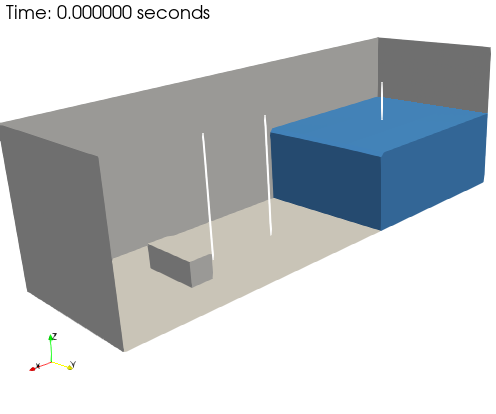
\includegraphics[height=2.0in]{images/3d_hex8_dam_break_geom.png}
  }
  \caption{Three-dimensional dam break geometry. Also shown are the experimental height probes that
are ordered from the obstruction backward, H1, H2, and H3.}
  \label{fig:geom}
\end{figure}

\section{Theory}
The air/water configuration is represented by the following set of 
transport equations,

Continuity:
\begin{align}
  \frac{ \partial u_j}{\partial x_j} = 0.
\label{eq:contEq}
\end{align} 

Momentum:
\begin{align}
  \frac {\partial \rho u_i }{\partial t} + \frac{ \partial \rho u_j u_i}{\partial x_j} 
-\frac{\partial \sigma_{ij}}{\partial x_j} = F_i.
\label{eq:momEq}
\end{align}

Volume of Fluid:
\begin{align}
  \frac{\partial \alpha}{\partial t} + u_j \frac{ \partial \alpha }{\partial x_j} = 0.
\label{eq:contEq}
\end{align} 

%
In the above equation, $\rho$ is the fluid density, $\alpha$ is the volume of fluid, 
and $u_j$ is the fluid velocity. 
The stress tensor is provided by
\begin{align}
\sigma_{ij}  = 2 \mu S^*_{ij} - P \delta_{ij},
\end{align}
%
where the traceless rate-of-strain tensor is defined as
\begin{align}
S^*_{ij}  = S_{ij} - \frac{1}{3} \delta_{ij} S_{kk} \nonumber
		     = S_{ij} - \frac{1}{3} \frac{\partial  u_k }{\partial x_k}\delta_{ij}.
\end{align}
The momentum equation includes the general source term $F_i$, which contains
both gravitational, $\rho g_i$, and surface tension 
effects, $\sigma \kappa \frac{\partial \alpha}{\partial x_i}$. Here, 
$\sigma$ is the surface tension of the liquid and $\kappa$ is the 
curvature, $\kappa = -\frac{\partial n_j}{\partial x_j}$, with the 
surface normal, $n_j$, defined as,

\begin{align}
  n_j = \frac{\frac{\partial \alpha}{ \partial x_j}} {\norm{\frac{\partial \alpha}{ \partial x_j}}},
\label{vofNorm}
\end{align}

In a low-Mach flow, the above pressure, $P$, is the perturbation about the thermodynamic
pressure, $P^{th}$. Surface tension can also be applied in this configuration.

Properties as a function of the volume of fluid via a linear relationship,
\begin{align}
\phi = \phi^L \alpha^L + \phi^G\left(1-\alpha \right),
\end{align}
where $\phi^L$ and $\phi^G$ are the properties at a pure liquid and gas state, respectively. Therefore,
$\alpha$ is interpreted at the volume fraction of liquid, where a value of unity implies pure liquid.
The isosurface of $1/2$ represents the diffuse interface between liquid and air.

The underlying methodology exercises a balanced-force method for pressure stabilization
in the presence of multi-phase flow, see Francois \textit{et al.}~\cite{francois2006} and
the more recent unstructured control-volume finite element method work of Domino and 
Horne~\cite{dominoHorne2022}.

\section{Results}
We follow the numerical validation approach of Kleefsman \textit{et al.}~\cite{kleefsman2005}
where prediction of water level heights at various stations and time are provided. These
data files are available in the postP directory.

\subsection{Simulation Specification and Results}

The density of air and water are specified to be 1 and 1000 $kg/m^3$, respectively,
while the viscosity for air and water are 1.98e-5 and 1.0e-3 $Pa-s$, respectively. The 
coarse mesh simulation exercises a Hex8 linear element.

In Figure~\ref{fig:results}, results are provided for the specifications
provided above.

\begin{figure}[!htbp]
  \centering
  {
   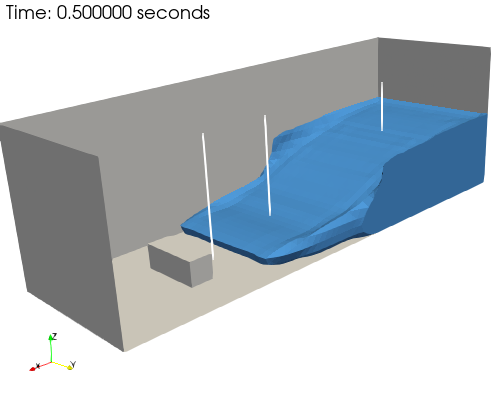
\includegraphics[height=1.2in]{images/results_0p50sec.png}
  }
  \centering
  {
   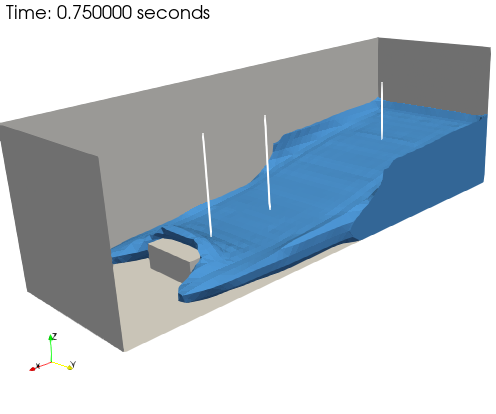
\includegraphics[height=1.2in]{images/results_0p75sec.png}
  }
  \centering
  {
   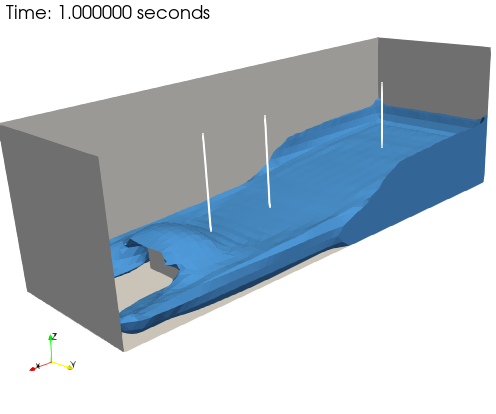
\includegraphics[height=1.2in]{images/results_1p0sec.png}
  } \\
  \centering
  {
   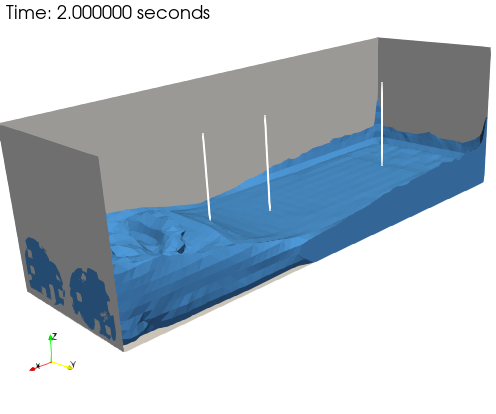
\includegraphics[height=1.2in]{images/results_2p0sec.png}
  }
  \centering
  {
   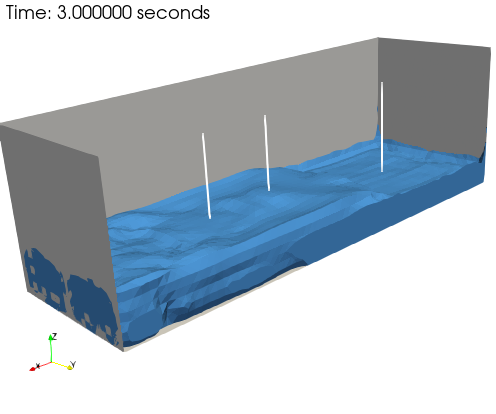
\includegraphics[height=1.2in]{images/results_3p0sec.png}
  }
  \centering
  {
   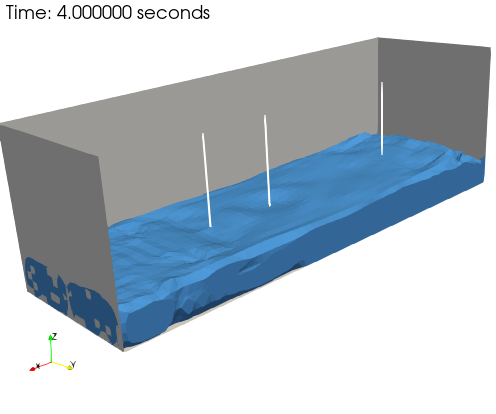
\includegraphics[height=1.2in]{images/results_4p0sec.png}
  }
  \caption{Volume of fluid evolution at 0.5, 0.75, 1.0, 2.0, 3.0, and 4.0 seconds.}
  \label{fig:results}
\end{figure}

\section{Discussion Points}

There are several interesting activities associated with this sample case including
the following:

\begin{itemize}
	\item Explore the mesh and input file specifications associated with this case.
	\item Replicate Figure~\ref{fig:results} using Paraview. Here, load the data set and perform a 
          ``clip'' based on the scalar value of volume of fluid to be one-half.
        \item Probe all degree-of-freedom results, i.e., velocity and pressure. What is of interest?
        \item Set the line command ``activate\_buoyancy\_pressure\_stabilization: no'', and add an
          additional source term to the momentum system by the name $buoyancy$. Re-run and report 
          and differences.
\end{itemize}

\begin{thebibliography}{100}

\bibitem{kleefsman2005} Kleefsman, K., Fekken, G., Veldman, A., Iwanowski, B., and Buchner, B., \emph{A balanced-force algorithm for continuous and sharp interfacial surface tension models within a volume tracking framework}, Journal of Computational Physics, Vol. 1, pp.141-173, 2006.

\bibitem{francois2006} Francois, M. M.,  Cummins, S. J.,  Dendy, E. D.,  Kothe, D. B.,  Sicilian, J. M., Williams, M. W., \emph{A Volume-of-Fluid based simulation method for wave impact problems}, Journal of Computational Physics, Vol. 1, pp.363-393, 2005.

\bibitem{dominoHorne2022} Domino, S. P., Horne, W., \emph{Development and deployment of a credible unstructured, six-DOF, implicit low-Mach overset high-fidelity simulation tool for wave energy applications}, Renewable Energy, under review, 2022.

\end{thebibliography}

\end{document}
